

\section{Approach}
\label{sec:model}
\figref{fig:model} gives an overview of the proposed model,
which is a three-way architecture: a user, a candidate concept, and paths from the user to the concept.
Given a user and a candidate concept, 
the model explores various paths connecting the user and concept in the concept net as context.
Leveraging rich features extracted from user behavior and profile, 
candidate concept schema, and path context, 
the model finally outputs a score, representing the probability of the user needs the candidate concept. 
To better improve the representations of three components and offer more interpretability, 
the attention cube is deployed to investigate complex mutual effects 
among user profile, path types and concept schema.
Now we present the proposed model \textbf{CptInfer}, which aims to INFER user needs (also known as ConcePT), in detail.

\begin{figure*}[th]
	\centering
	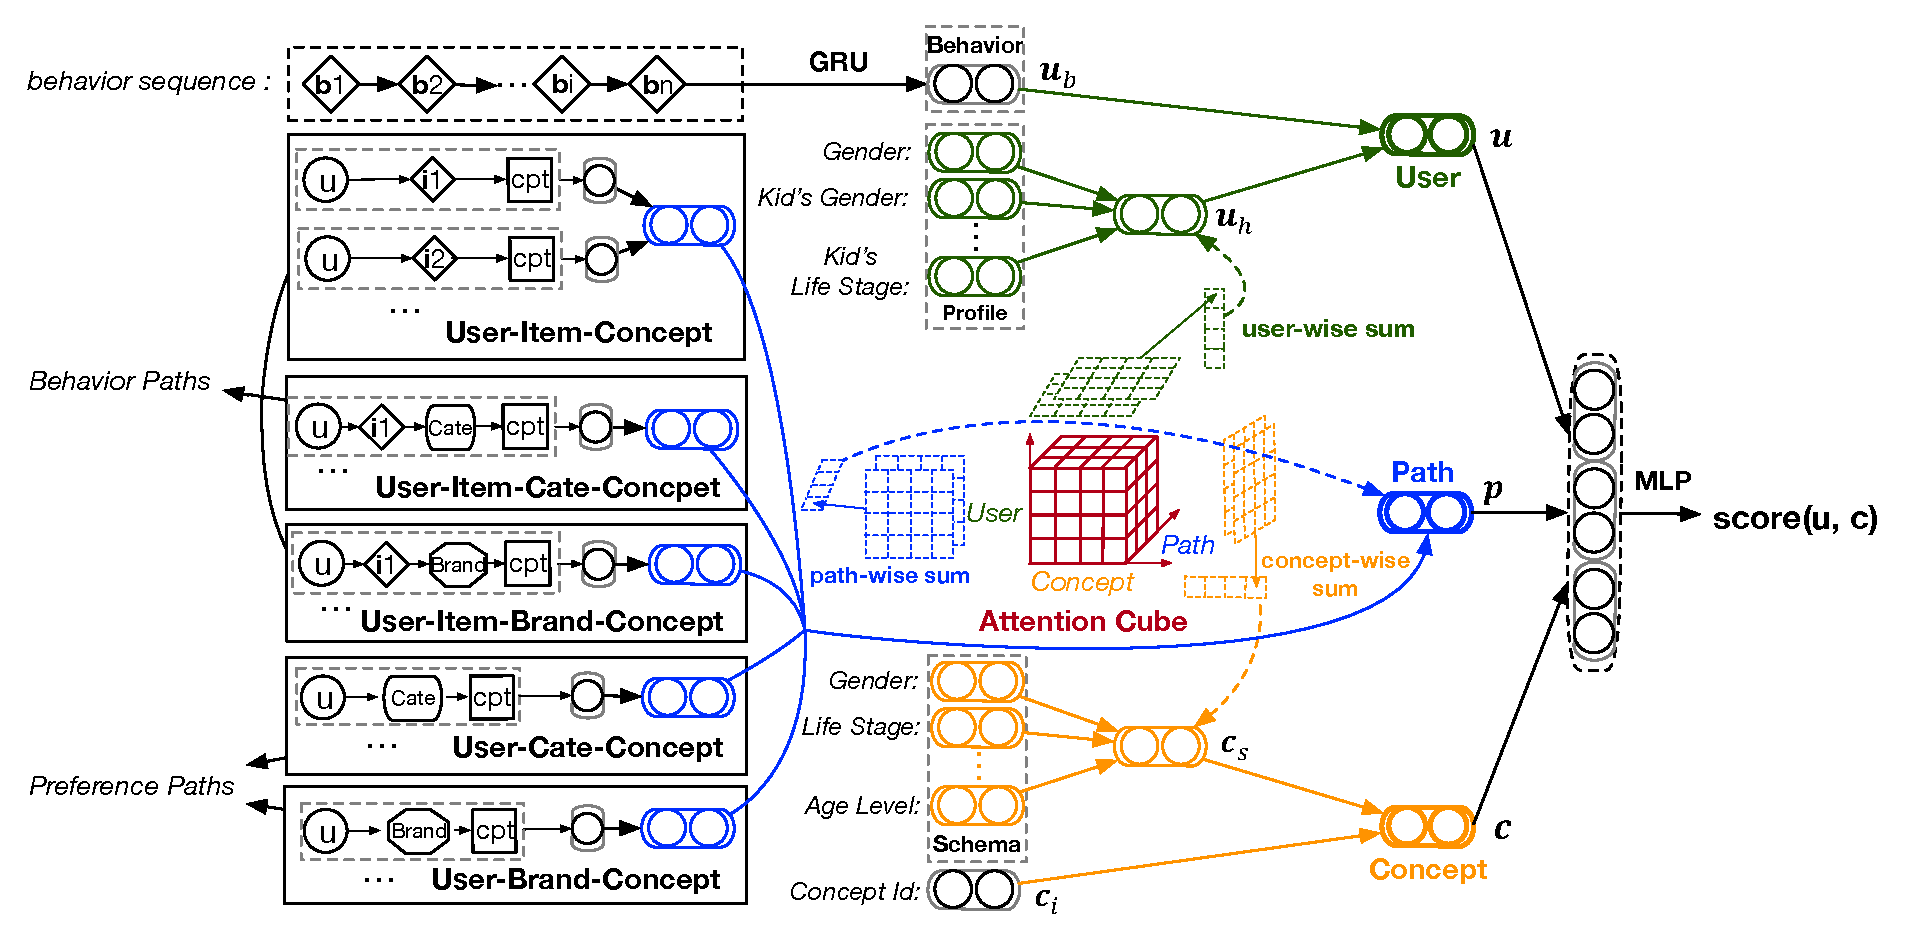
\epsfig{file=figures/model.eps, width=2\columnwidth}
	\caption{Overview of proposed model.}
	\label{fig:model}
\end{figure*}

\subsection{User Embedding}

The representation for each user comes from two parts: user behavior sequence and user profile.

\noindent
\textbf{User Behavior Sequence}

\noindent
Each behavior consists of three things: the item, the behavior type and the behavior time.
Due to enormous amount of items (over 1 billion) in e-commerce platform, 
we represent each item in behavior sequence 
using its description such as category, brand and shop, instead of directly using its id.
This is for two reasons: to save memory for storing large amount of id embeddings and to avoid sparsity problem when encountering long-tail or new items while predicting.
We consider four types of behavior: \textit{click}, \textit{bookmark}, \textit{add to cart} and \textit{purchase}.
In addition, the day gap between the behavior and current time is also taken into account. 
Therefore, each behavior $b_i$ can be represented as a multi-hot vector 
$[\bi{b}_{i}^{1}, \bi{b}_{i}^{2}, \cdots, \bi{b}_{i}^{F}]$,
where each one-hot vector $\bi{b}_{i}^{f}$ corresponds to one of the above mentioned feature and $F$ is the total number.
Then an embedding lookup layer shown in \figref{fig:detail_2} maps
sparse behavior vector into a low-dimensional dense vector  $\bi{b}_i$:

\begin{equation}
\label{eqn:lookup}
\bi{b}_i = [\bi{W}_{lk}^{1}\bi{b}_{i}^{1}; \bi{W}_{lk}^{2}\bi{b}_{i}^{2}; \cdots; \bi{W}_{lk}^{F}\bi{b}_{i}^{F}],
\bi{W}_{lk}^{f} \in \bi{R}^{d^{f} \times V^{f}} 
\end{equation}

\noindent
where $\bi{W}_{lk}^{f}$ are parameters for embedding lookup layer,
$d^{f}$ is the dimension of dense vector and $V^{f}$ is the vocabulary size.


\begin{figure}[th]
	\centering
	\epsfig{file=figures/model_detail_2.eps, width=\columnwidth}
	\caption{Encoding of user behavior}
	\label{fig:detail_2}
\end{figure}

Recurrent neural Networks (RNN) have been proven effective in capturing temporal dependency in sequence data.
%A major challenge of RNNs is that it suffers from the problem of ``gradient vanishing'' while handling long sequences.
%To alleviate this problem, two variants, namely the Long Short Term Memory (LSTM) networks \cite{hochreiter1997long} and Gated Recurrent Unit (GRU) networks \cite{cho2014properties} are proposed. 
We adopt the GRU \cite{cho2014properties} networks, a variant of RNN, as the behavior sequence encoder
since it is able to handle long sequences than normal RNN.
Then embedding of user behavior sequence $\bi{u}_b$ is calculated as:
\begin{equation}
\bi{u}_b = GRU(\bi{b}_1, \bi{b}_2, \cdots, \bi{b}_n)
\end{equation}

\noindent
\textbf{User Profile}

\noindent
The aspects of user profile include \textit{gender}, \textit{age level}, \textit{kid's gender}, \textit{kid's life stage}, etc.
We use a simple lookup layer similar to \eqnref{eqn:lookup} to obtain the corresponding embedding for each profile aspect.
Then we apply a function $f_{u}$ to map the embedding list 
$u_h = [\bi{h}_{\text{gender}}, \bi{h}_{\text{age}}, \cdots]$ to a single vector as the representation of user profile $\bi{u}_p$:
\begin{equation}
\label{eqn:fu}
\bi{u}_h = f_u(u_h) = f_u([\bi{h}_{\text{gender}}, \bi{h}_{\text{age}}, \cdots])
\end{equation}
where the simplest $f_u$ is average pooling. Optimizations for $f_u$ will be discussed in \secref{sec:att}.

Finally we get the user embedding $\bi{u}$ by concatenation plus a fully connected layer:
\begin{equation}
\bi{u} = \textbf{FC}([\bi{u}_{b};\bi{u}_{h}])
\end{equation}

\subsection{Concept Embedding}

Similar to user embedding which comes from user behavior and user profile, we use two components to encode the candidate concept: concept id and concept schema.
The representation of concept id $\bi{c}_i$ is obtained simply by lookup.
For concept schema,
we use embedding lookup layer to map one-hot vectors (aspects of concept schema) to dense vectors, then apply function $f_{c}$ to obtain
the representation of the concept schema $\bi{c}_s$. 
Similar to the encoding of user profile,
we then obtain concept embedding $\bi{c}$ :
\begin{equation}
\label{eqn:fc}
\bi{c}_s = f_c(c_s) = f_c([\bi{s}_{\text{gender}}, \bi{s}_{\text{age}}, \cdots])
\end{equation}
\begin{equation}
\bi{c} = \textbf{FC}([\bi{c}_{i};\bi{c}_{s}])
\end{equation}

\subsection{Path Embedding}
\label{sec:path}
In order to leverage rich semantic features from the e-commerce concept net,
we explore paths connecting users and concepts within the graph.
We adopt the idea of \textit{meta-path} \cite{hu2018leveraging}, due to the fact KGs in e-commerce are usually extremely large.
If we let the model discover possible paths from a behaved item to a concept freely as described in RippleNet \cite{wang2018ripplenet}, 
the computational overhead is unacceptable.
Besides, empirical experience is valuable in e-commerce.
Therefore, we believe manually crafted meta-paths are able to reduce noises and improve efficiency.
A meta-path is a path in the form of ``$T_1 \rightarrow T_2 \rightarrow \cdots T_n$'', where each node (exclude user in our case) is a type of entity in the concept net, such as ``$User \rightarrow Item \rightarrow Category \rightarrow Concept$''.
We mainly consider two types of meta-path in our concept net: \textit{behavior} path and \textit{preference} path.
Behavior paths are triggered by items which a user clicks or purchases, such as ``\textbf{UIC}'' (User-Item-Concept), and  ``\textbf{UITC}''(``\textbf{T}'' for ``Ca\textbf{T}egory'').
Preference paths are triggered by long-term preferred categories or brands, such as ``\textbf{UBC}''(``\textbf{B}'' for ``\textbf{B}rand'').

Within each meta-path, 
there are multiple specific paths called \textit{path instance}s.
For each meta-path, we sample a fixed number of path instances with highest priority scores.
Calculation of the priority score for each edge in a path instance is based on heuristics.
In the concept net, one item may belong to several concepts, while each concept also contains many items. So we mainly adopt \textit{tf-idf} score to measure the importance of each ``item-concept'' edge and other types of edge.
The score of the whole path instance is then calculated as the product of all the edge scores.
Then we use a Convolution Neural Network (CNN) to encode each sampled instance $\bi{pi}$ and followed by a max-pooling operation to get the embedding of that meta-path
(take ``\textbf{UITC}'' as an example):
\begin{equation}
\label{eqn:cnn}
\bi{pi}_{\text{UITC}} =  \textbf{CNN}([\bi{u}_b, \bi{i}, \bi{cate}, \bi{c}_i])
\end{equation}
\begin{equation}
\bi{p}_{\text{UITC}} = \textbf{MaxPooling}(\{\bi{pi}_{\text{UITC}}\})
\end{equation}
where $\bi{i}$ is the item embedding which only uses item description, 
and $\bi{cate}$ is id lookup embedding of category. As for head and tail node, $\bi{u}_b$ is the behavior embedding and $\bi{c}_i$ is the lookup embedding of concept id.
Comparing to RNN, CNN is much faster dealing with large amount of data and able to extract sequence dependency when sequence length is relatively short.
Then the representation of meta-path context is calculated as:
\begin{equation}
\label{eqn:fp}
\bi{p} = f_p(p) = f_p(\bi{p}_{\text{UIC}}, \bi{p}_{\text{UITC}}, \cdots)
\end{equation}


\subsection{The Whole Model}

After getting the embedding for the user, the candidate concept and the paths connecting them, we concatenate the three embeddings and feed it into a MLP and the final output indicates the probability user $u$ will need concept $c$:
\begin{equation}
\hat y_{uc} = \textbf{MLP}([\bi{u};\bi{p};\bi{c}]),
\end{equation}
where the MLP module consists of two hidden layers with ReLU activation function and an output layer with sigmoid function.

We interpret user needs inference as a binary classification problem, 
where an observed user-concept interaction is assigned with a target value $1$, otherwise $0$. 
We use point-wise learning with the negative log-likelihood objective function to learn the parameters of our model:
\begin{equation}
\mathscr{L} = -\sum_{(u, c)\in D^+}{\log \hat y_{uc}} + \sum_{(u, c)\in D^-}{\log (1-\hat y_{uc})}
\end{equation}
where $D^+$ and $D^-$ are the positive and negative user-concept interaction pairs.


\subsection{Attention Mechanism}
\label{sec:att}

%Intuitively, different paths are likely to effect users' decision making differently. Even for the same user, the preference on the same path may change targeting different concepts.
If we define $f_u$, $f_c$ and $f_p$ as average pooling functions, each element contributes equally all the time.
It is obviously suboptimal since different meta-paths are likely to effect users' decision making differently.
Even for the same user, the preference on the same path may change targeting different concepts.
Similarly, different aspects of user profile and concept schema can contribute to the final decision differently as well.
For example, a pregnant female user is more likely to be in need of a concept like ``Snacks for Pregnancy'' rather than ``Primary School''.
Some concepts are originally designed for a target group of users, so that different aspects should be weighted differently
when encoding the user or the concept in each interaction.
It is vital to investigate the mutual influence among 
user profile aspects, concept schema aspects and different mate-paths,
since the input of our problem are much more informative comparing to previous works \cite{hu2018leveraging,wang2018ripplenet,wang2018explainable}.

Attention mechanism has been been widely used to handle weighted sum of embeddings 
in recent years \cite{bahdanau2014neural,yin2016abcnn}.
We proposed a novel attention module called ``\textbf{Attention Cube}'' to 
model the mutual influence of a three way interaction simultaneously in our problem.
Attention cube is a three-dimensional tensor with $x$, $y$, $z$ axis corresponding to $user$, $path$ and $concept$. 
We extend Luong's attention equation \cite{luong2015effective} to three-dimension and define the values of attention cube $\bi{Att}$ as below:
\begin{equation}
\label{eqn:att}
att_{i,j,k} = {{u_h}_i}^T \bm{W_1} h_j + {p_j}^T \bm{W_2} {c_s}_k + {{u_p}_i}^T \bm{W_3} {c_s}_k  
\end{equation}
where ${u_h}_i$ is $i^{th}$ embedding of user profile embedding list,
 ${c_s}_k$ is $k^{th}$ embedding of concept schema embedding list,
 and $p_j$ is $j^{th}$ embedding of meta-path embedding list.
 $\bm{W_1}$,  $\bm{W_2}$,  $\bm{W_3}$ are parameter matrices.
 
Then the weights of user profile aspects, concept schema aspects and different meta-paths are obtained by first calculating axis-wise sum and then normalization:
\begin{equation}
{\bm{\alpha_u}}_i = \frac{\exp(\sum_{j}\sum_{k} att_{i,j,k})}{\sum_{i}exp(\sum_{j}\sum_{k} att_{i,j,k})}
\end{equation}

We can get ${\bm{\alpha_p}}_j$ and ${\bm{\alpha_c}}_k$ in a similar way.
Finally, the mapping functions $f_u$ (similar for $f_c$ and $f_p$) are defined to get $\bi{u}_h$ (similar for $\bi{c}_s$ and $\bi{p}$) as below:
\begin{equation}
\bi{u}_h = f_u(u_h) = {\bm{\alpha_u}}_1 \bi{h}_{\text{gender}} + {\bm{\alpha_u}}_2 \bi{h}_{\text{age}} + \cdots 
\end{equation}

Since the attention weights ${\bm{\alpha_u}}_i$, ${\bm{\alpha_p}}_j$ and ${\bm{\alpha_c}}_k$ are generated for each user-concept interaction separately, they are able to capture the complex mutual influence among the three components and result in better representations.

 
 
 


